%\chapter\veeesults}

%\section{Problem A: Pathfinding in 2D Games}

All deliverables in the form of code are enclosed.

\subsection*{Subproblem A.1: Grids with Obstacles}

The following figures show the solution path calculated by the A* implementation,
with the $\text{OPEN}$ and $\text{CLOSED}$ sets visualized as respectively cyan
and pink dots.

\begin{figure}[h!]
  \centering
    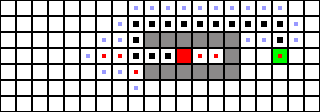
\includegraphics[width=0.8\textwidth]{img/board-1-1-astar}
    \caption{Board 1.1}
\end{figure}

\begin{figure}[h!]
  \centering
    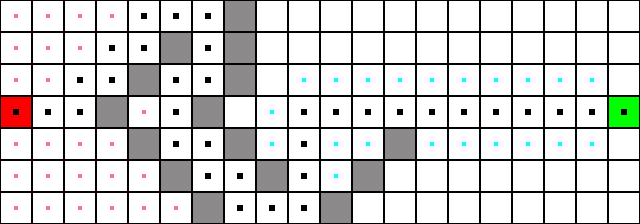
\includegraphics[width=0.8\textwidth]{img/board-1-2-astar}
    \caption{Board 1.2}
\end{figure}

\begin{figure}[h!]
  \centering
    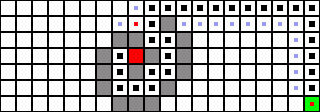
\includegraphics[width=0.8\textwidth]{img/board-1-3-astar}
    \caption{Board 1.3}
\end{figure}

\begin{figure}[h!]
  \centering
    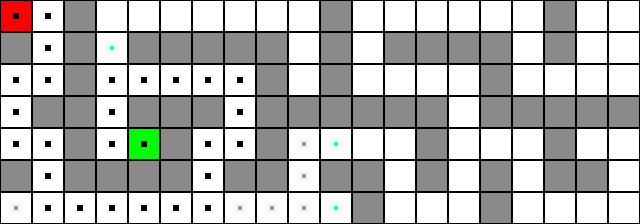
\includegraphics[width=0.8\textwidth]{img/board-1-4-astar}
    \caption{Board 1.4}
\end{figure}

\clearpage

\subsection*{Subproblem A.2: Grids with different cell costs}

For this subproblem, we modified our implementation to be able to parse weighted
boards as well as correctly handling cost calculation of weighted nodes.
Again, the visualizations include the $\text{OPEN}$ and $\text{CLOSED}$ sets.

\begin{figure}[h!]
  \centering
    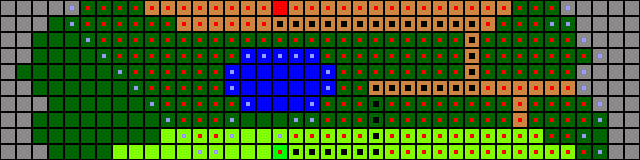
\includegraphics[width=\textwidth]{img/board-2-1-astar}
    \caption{Board 2.1}
\end{figure}

\begin{figure}[h!]
  \centering
    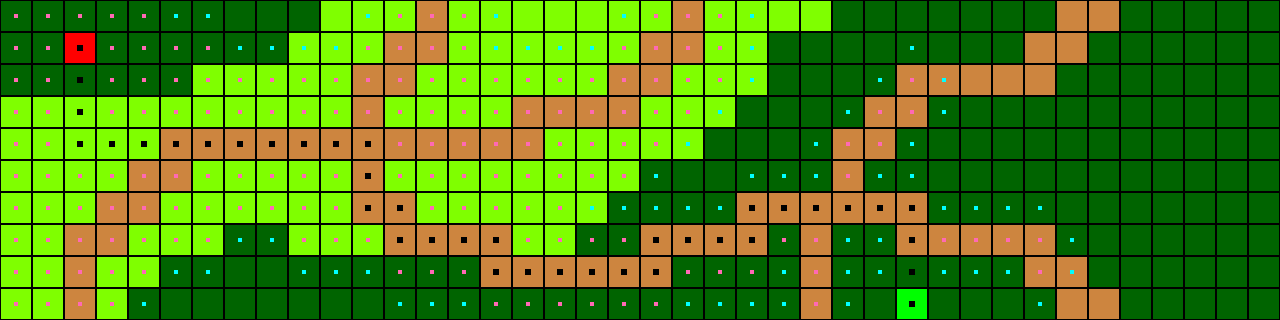
\includegraphics[width=\textwidth]{img/board-2-2-astar}
    \caption{Board 2.2}
\end{figure}

\begin{figure}[h!]
  \centering
    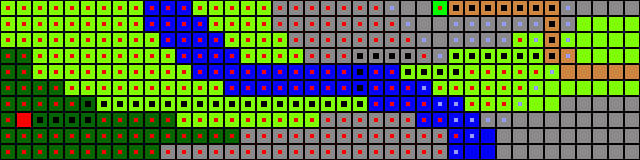
\includegraphics[width=\textwidth]{img/board-2-3-astar}
    \caption{Board 2.3}
\end{figure}

\begin{figure}[h!]
  \centering
    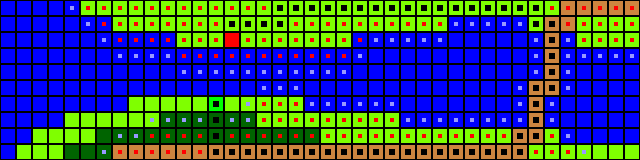
\includegraphics[width=\textwidth]{img/board-2-4-astar}
    \caption{Board 2.4}
\end{figure}

\clearpage

\subsection*{Comparison with BFS and Dijkstra's Algorithm}

\subsubsection*{Board 1.1}

\begin{figure}[h!]
  \centering
    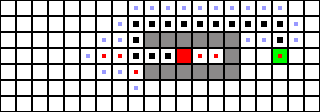
\includegraphics[width=0.8\textwidth]{img/board-1-1-astar}
    \caption{Board 1.1 - A*}
\end{figure}

\begin{figure}[h!]
  \centering
    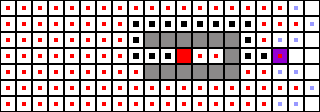
\includegraphics[width=0.8\textwidth]{img/board-1-1-dijkstra}
    \caption{Board 1.1 - Dijkstra}
\end{figure}

\begin{figure}[h!]
  \centering
    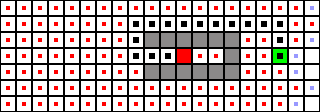
\includegraphics[width=0.8\textwidth]{img/board-1-1-bfs}
    \caption{Board 1.1 - BFS}
\end{figure}

All three algorithms find an equally short path, but A* examines significantly
fewer nodes doing it.

\clearpage

\subsubsection*{Board 1.2}

\begin{figure}[h!]
  \centering
    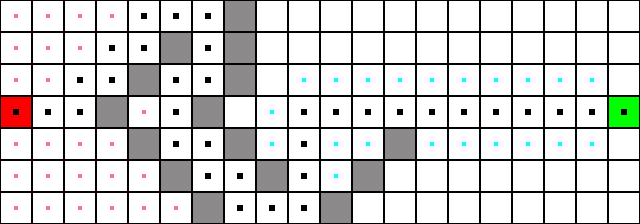
\includegraphics[width=0.8\textwidth]{img/board-1-2-astar}
    \caption{Board 1.2 - A*}
\end{figure}

\begin{figure}[h!]
  \centering
    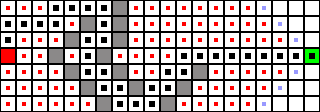
\includegraphics[width=0.8\textwidth]{img/board-1-2-dijkstra}
    \caption{Board 1.2 - Dijkstra}
\end{figure}

\begin{figure}[h!]
  \centering
    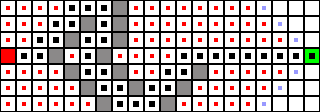
\includegraphics[width=0.8\textwidth]{img/board-1-2-bfs}
    \caption{Board 1.2 - BFS}
\end{figure}

All algorithms find the shortest path, but again, A* is much more efficient.

\clearpage

\subsubsection*{Board 1.3}

\begin{figure}[h!]
  \centering
    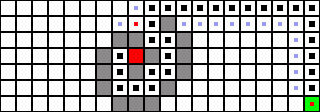
\includegraphics[width=0.8\textwidth]{img/board-1-3-astar}
    \caption{Board 1.3 - A*}

\end{figure}

\begin{figure}[h!]
  \centering
    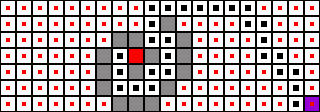
\includegraphics[width=0.8\textwidth]{img/board-1-3-dijkstra}
    \caption{Board 1.3 - Dijkstra}
\end{figure}

\begin{figure}[h!]
  \centering
    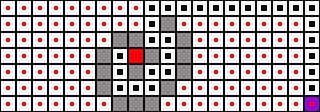
\includegraphics[width=0.8\textwidth]{img/board-1-3-bfs}
    \caption{Board 1.3 - BFS}
\end{figure}

Again, A* is much more efficient than the others.

\clearpage

\subsubsection*{Board 1.4}

\begin{figure}[h!]
  \centering
    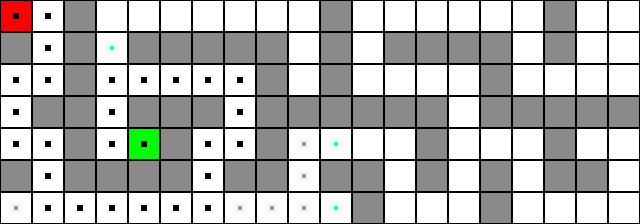
\includegraphics[width=0.8\textwidth]{img/board-1-4-astar}
    \caption{Board 1.4 - A*}
\end{figure}

\begin{figure}[h!]
  \centering
    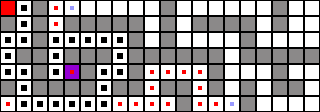
\includegraphics[width=0.8\textwidth]{img/board-1-4-dijkstra}
    \caption{Board 1.4 - Dijkstra}
\end{figure}

\begin{figure}[h!]
  \centering
    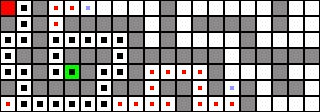
\includegraphics[width=0.8\textwidth]{img/board-1-4-bfs}
    \caption{Board 1.4 - BFS}
\end{figure}

For this board, we see that there's not much difference between the three
algorithms. A* explores marginally fewer nodes than the other two.

\clearpage

\subsubsection*{Board 2.1}

\begin{figure}[h!]
  \centering
    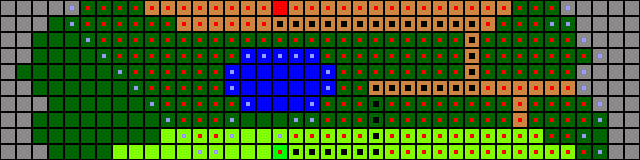
\includegraphics[width=\textwidth]{img/board-2-1-astar}
    \caption{Board 2.1 - A*}
\end{figure}

\begin{figure}[h!]
  \centering
    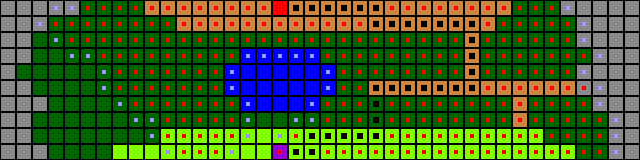
\includegraphics[width=\textwidth]{img/board-2-1-dijkstra}
    \caption{Board 2.1 - Dijkstra}
\end{figure}

\begin{figure}[h!]
  \centering
    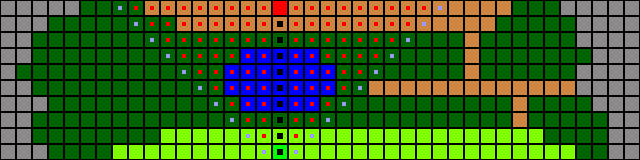
\includegraphics[width=\textwidth]{img/board-2-1-bfs}
    \caption{Board 2.1 - BFS}
\end{figure}

For this board, we see that A* and Djikstra both find equally optimal paths,
both processing about the same number of nodes. (A* slightly lower as the 
heuristic is taken into consideration.) BFS processes fewer nodes, but finds an
extremely unoptimized path.

\clearpage

\subsubsection*{Board 2.2}

\begin{figure}[h!]
  \centering
    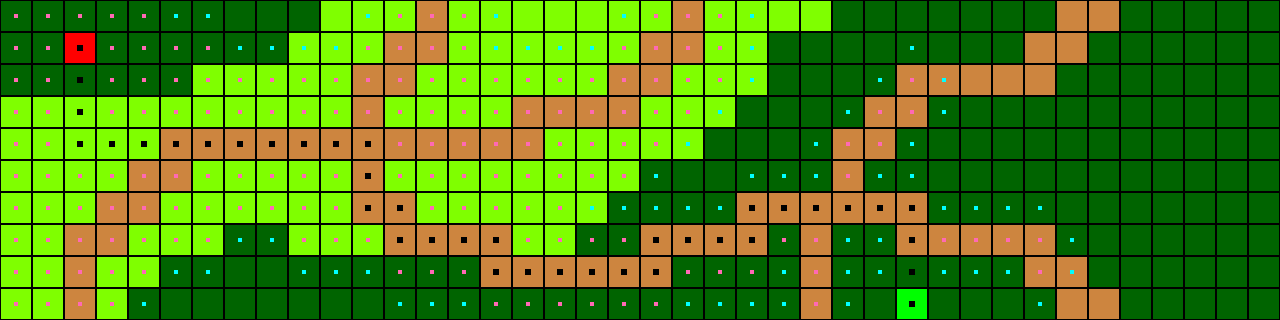
\includegraphics[width=\textwidth]{img/board-2-2-astar}
    \caption{Board 2.2 - A*}
\end{figure}

\begin{figure}[h!]
  \centering
    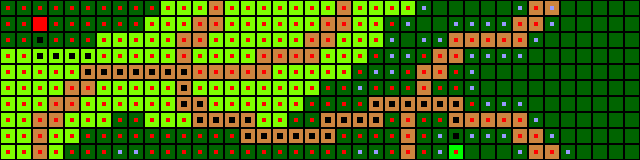
\includegraphics[width=\textwidth]{img/board-2-2-dijkstra}
    \caption{Board 2.2 - Dijkstra}
\end{figure}

\begin{figure}[h!]
  \centering
    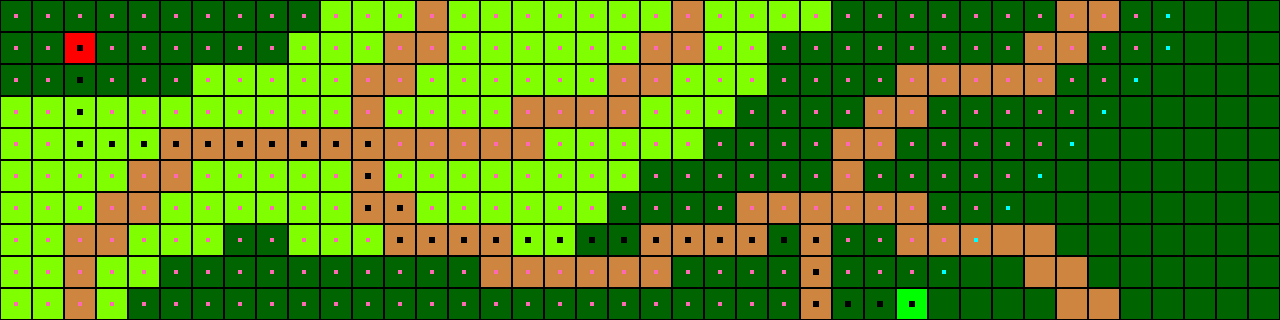
\includegraphics[width=\textwidth]{img/board-2-2-bfs}
    \caption{Board 2.2 - BFS}
\end{figure}

A* and Dijkstra both perform reasonably well here, while BFS makes quite a few
suboptimal choices while also processing more nodes.

For the case of A* vs. Djikstra, we see that A* (as it should) refrains from
processing nodes that have low cell weight, but also have higher heuristic values.

\clearpage

\subsubsection*{Board 2.3}

\begin{figure}[h!]
  \centering
    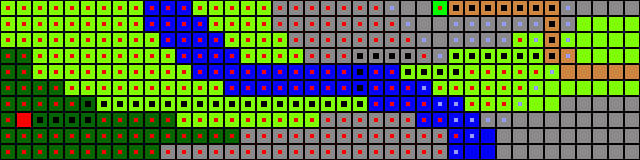
\includegraphics[width=\textwidth]{img/board-2-3-astar}
    \caption{Board 2.3 - A*}
\end{figure}

\begin{figure}[h!]
  \centering
    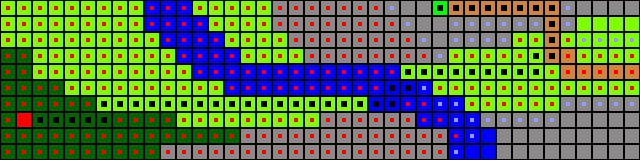
\includegraphics[width=\textwidth]{img/board-2-3-dijkstra}
    \caption{Board 2.3 - Dijkstra}
\end{figure}

\begin{figure}[h!]
  \centering
    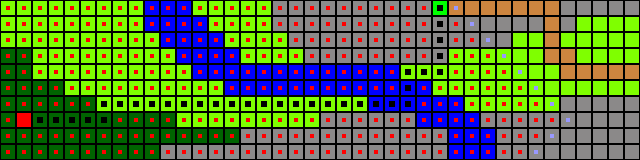
\includegraphics[width=\textwidth]{img/board-2-3-bfs}
    \caption{Board 2.3 - BFS}
\end{figure}

Again, A* and Dijkstra both find equally optimal paths, while BFS naively picks
the first path it can find.

\clearpage

\subsubsection*{Board 2.4}

\begin{figure}[h!]
  \centering
    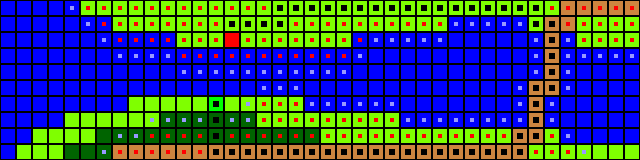
\includegraphics[width=\textwidth]{img/board-2-4-astar}
    \caption{Board 2.4 - A*}
\end{figure}

\begin{figure}[h!]
  \centering
    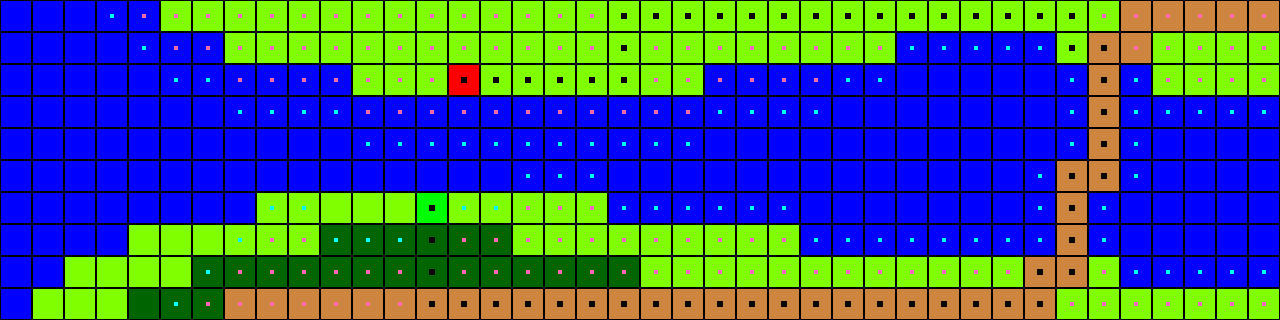
\includegraphics[width=\textwidth]{img/board-2-4-dijkstra}
    \caption{Board 2.4 - Dijkstra}
\end{figure}

\begin{figure}[h!]
  \centering
    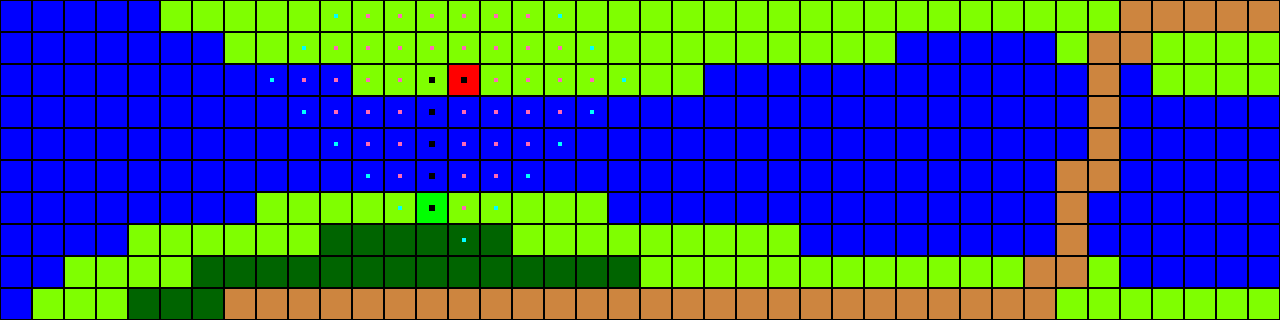
\includegraphics[width=\textwidth]{img/board-2-4-bfs}
    \caption{Board 2.4 - BFS}
\end{figure}

For this final board, A* and Dijkstra find the same path. A* processes slightly
fewer nodes, notably those in the bottom right corner of the board.
BFS processes few nodes, but finds a suboptimal path.


\section*{1}
\begin{enumerate}
    \item
        \begin{table}[h]
            \centering
            \begin{tabular}{l|l|l|l|l|l}
                \hline
                1,3 & 2,2 & 3,1 & KB & $\alpha_2$ & $\alpha_3$ \\\hline
                ~  & ~  & ~  & ~ & T & ~ \\
                P  & ~  & ~  & ~ & T & ~ \\
                W  & ~  & ~  & ~ & T & T \\
                PW & ~  & ~  & ~ & T & T \\
                ~  & P  & ~  & ~ & ~ & ~ \\
                P  & P  & ~  & ~ & ~ & ~ \\
                W  & P  & ~  & ~ & ~ & T \\
                PW & P  & ~  & ~ & ~ & T \\
                ~  & W  & ~  & ~ & T & ~ \\
                P  & W  & ~  & ~ & T & ~ \\
                ~  & PW & ~  & ~ & ~ & ~ \\
                P  & PW & ~  & ~ & ~ & ~ \\
                ~  & ~  & P  & ~ & T & ~ \\
                P  & ~  & P  & ~ & T & ~ \\
                W  & ~  & P  & T & T & T \\
                PW & ~  & P  & ~ & T & T \\
                ~  & P  & P  & ~ & ~ & ~ \\
                P  & P  & P  & ~ & ~ & ~ \\
                W  & P  & P  & ~ & ~ & T \\
                PW & P  & P  & ~ & ~ & T \\
                ~  & W  & P  & ~ & T & ~ \\
                P  & W  & P  & ~ & T & ~ \\
                ~  & PW & P  & ~ & ~ & ~ \\
                P  & PW & P  & ~ & ~ & ~ \\
                ~  & ~  & W  & ~ & T & ~ \\
                P  & ~  & W  & ~ & T & ~ \\
                ~  & P  & W  & ~ & ~ & ~ \\
                P  & P  & W  & ~ & ~ & ~ \\
                ~  & ~  & PW & ~ & T & ~ \\
                P  & ~  & PW & ~ & T & ~ \\
                ~  & P  & PW & ~ & ~ & ~ \\
                P  & P  & PW & ~ & ~ & ~ \\
            \end{tabular}
            \caption {Wumpus}
        \end{table}
        We can see that $\text{KB} \models \alpha_2$ and $\text{KB} \models \alpha_3$ since the single row with $\text{KB} = \text{True}$ has both $\alpha_2$ and $\alpha_3$ True.

    \item

        \begin{enumerate}[a.]
            \item True, False is never true, ergo this statement doesn't violate the definition of entailment.
            \item False. Inverse of above, False is never true, and the statement will therefore always violate the definition.
            \item True. $M(\text{LHS}) \subseteq M(\text{RHS})$
            \item False. With both $A$ and $B$ True, the LHS will be true, but the RHS will be false. Thus $M(\text{LHS}) \not\subseteq M(\text{RHS})$.
            \item True. $M(\text{LHS}) = M(\text{RHS})$ for this statement.
            \item True. The only case that would make the right hand side False is $A = B = \text{True}, C = False$ for which the LHS is also false.
        \end{enumerate}
    \item
        \begin{enumerate}[a.]
            \item $\{T, F\}, \{TF, FT, TT\}, \{T, F\}$. $2*3*2 = 12$
            \item Only false if all propositions are True, therefore $2^4 - 1 = 15$ models.
            \item $0$. $A = T, B = F$ means that $A \implies B$ can never be true.
        \end{enumerate}

    \item
        \begin{enumerate}[a.]
            \item Valid. $\text{Smoke} \implies \text{Smoke} \equiv \neg \text{Smoke} \vee \text{Smoke}$
            \item Neither. All models except $\text{Smoke} = \text{True}, \text{Fire} = \text{False}$ satisfies the sentence.
            \item Neither. 
                \begin{gather*}
                    (\text{Smoke} \implies \text{Fire}) \implies (\neg \text{Smoke} \implies \neg \text{Fire})
                    \equiv (\neg \text{Smoke} \vee \text{Fire} \implies \neg \text{Fire} \vee \text{Smoke})
                \end{gather*}
                False for $\text{Smoke} = \text{False}, \text{Fire} = \text{True}$
        \end{enumerate}
    \item
        \begin{enumerate}[a.]
            \item $^3/_4 Q$
            \item $^5/_8 Q$
            \item $^3/_4 Q$
        \end{enumerate}
\end{enumerate}

\section*{2}
\subsection*{1}
\begin{enumerate}
    \item $A \wedge B \wedge C$
    \item $A \vee B \vee C$
    \item $\neg A \vee B \vee C$
    \item $(\neg A \vee C) \wedge (B \vee C)$
    \item $\neg A \vee \neg B \vee C \vee D$
    \item $(\neg A \vee C) \wedge (\neg A \vee D) \wedge (\neg B \vee C) \wedge (\neg B) \vee D)$
    \item $(\neg A \vee \neg B \vee C) \wedge (A \vee \neg C) \wedge (B \vee \neg C)$
\end{enumerate}
\subsection*{2}
The items in the KB individually CNF to:
\begin{itemize}
    \item   $(\neg A \vee  \neg C) \wedge  (B \vee  \neg C)$
    \item   $(C \vee  \neg E) \wedge  D$
    \item   $A \wedge D$
\end{itemize}

Since these statements are the KB, we can and them together, and simplify:
\begin{align*}
(\neg A \vee  \neg C) \wedge  (B \vee  \neg C) \wedge (C \vee  \neg E) \wedge  D \wedge A \wedge D
\\
(\neg A \vee  \neg C) \wedge  (B \vee  \neg C) \wedge (C \vee  \neg E) \wedge  D \wedge A
\\
\neg C \wedge  (B \vee  \neg C) \wedge (C \vee  \neg E) \wedge  D \wedge A
\\
\neg C \wedge  B \wedge \neg E \wedge  D \wedge A
\end{align*}
And at this point we can see that for the KB to hold true, we must have $\neg E$.


\section*{3}
\subsection*{1}
\begin{enumerate}[a.]
    \item $\text{Occupation}(\text{Emily}, \text{Lawyer}) \vee \text{Occupation}(\text{Emily}, \text{Surgeon})$
    \item $\text{Occupation}(\text{Joe}, \text{Actor}) \wedge \exists o \{\text{Occupation}(\text{Joe}, o)\}$
    \item $\forall x \{\text{Occupation}(x, Doctor) \wedge \text{Occupation}(x, Surgeon)\}$
\end{enumerate}

\subsection*{2}
\begin{enumerate}[a.]
    \item $\forall x \{ \text{Even}(x) \Leftrightarrow \exists y \{ x = y + y\}\}$
    \item $\forall x \{ \text{Prime}(x) \Leftrightarrow \forall yz \{ x = y \times z \implies z = 1 \vee y = 1\}\}$
    \item $\forall x \{ \text{Even}(x) \Leftrightarrow \exists yz \{ x = y + z \wedge (\text{Prime}(y) \wedge \text{Prime}(z))\}\}$
\end{enumerate}

\subsection*{3}
\begin{gather*}
    \forall k \{ \text{Key}(k) \implies \exists t_0 \{\text{Before}(\text{Now}, t_0) \wedge \forall t \{ \text{Before}(t_0, t) \implies \text{Lost}(k, t)\} \} \\
    \forall xy \{ \text{Sock}(x) \wedge \text{Sock}(y) \wedge \text{Pair}(x, y) \implies \\
    \exists t_1 \{ \text{Before}(Now, t_1) \wedge \forall t \{ \text{Before}(t_1, t) \wedge \text{Lost}(x, t)\} \} \vee \\
    \exists t_2 \{ \text{Before}(Now, t_2) \wedge \forall t \{ \text{Before}(t_2, t) \wedge \text{Lost}(y, t)\} \} \}
\end{gather*}

\subsection*{4}
With the following vocabulary:
\begin{gather*}
    V = \{\text{Person}(x), \text{IsDNAOfPerson}(x, y), \text{IsParentOf}(x, y), \text{IsDerivedFromPersonsDNA}(x, y)\}
\end{gather*}

where $\text{Person}(x)$ is true if $x$ is a person, $\text{IsDNAOfPerson}(x, y)$ is true if $y$ is person $x$'s DNA, $\text{IsParentOf}(x, y)$ is true if $y$ is $x$'s parent and $\text{IsDerivedFromPersonsDNA}(x, y)$ is true if DNA $x$ is derived from person $x$'s DNA.
\begin{gather*}
    \forall xy \{ \text{Person}(x) \wedge \text{IsDNAOfPerson}(y, x) \implies \neg \exists z \{ \text{Person}(z) \wedge \text{IsDNAOfPerson}(y, z) \} \wedge \\
    \forall a \{ \text{Person}(a) \wedge \text{IsParentOf}(x, a) \implies \text{IsDerivedFromPersonsDNA}(y, a) \}\}
\end{gather*}


\section*{4}
\subsection*{1}
\begin{enumerate}[a.]
    \item $\Theta = \{x/\text{Rocky}\}$
    \item $\Theta = \{x/\text{Leo}, y/\text{Rocky}\}$
    \item $\Theta = \{x/\text{Rocky}, y/\text{Leo}\}$
    \item Not possible.
    \item Not Possible.
    \item $\Theta = \{x/\text{Leo}, y/\text{FastestHorse(x)}\}$
    \item $\Theta = \{x/\text{Marvin}, y/\text{Leo}\}$
\end{enumerate}

\subsection*{2}

Only the last sentence needs to be converted to CNF.

\begin{gather*}
    \forall x \{ \text{Green}(x) \leftrightarrow \text{Bikes}(x) \vee \exists y \{ \text{Drives}(x, y) \wedge \text{Hybrid}(y) \} \}
\end{gather*}
